\documentclass[aspectratio=169]{beamer}

% --- THEME ---
\usetheme{Madrid}
\usecolortheme{seahorse}
\setbeamertemplate{navigation symbols}{}
\setbeamertemplate{footline}[frame number]
\setbeamercolor{frametitle}{bg=structure.fg!15!bg}

\usepackage[utf8]{inputenc}
\usepackage[T1]{fontenc}
\usepackage{booktabs}
\usepackage{graphicx}
\usepackage{tikz}
\usetikzlibrary{shapes.geometric, arrows.meta, positioning, fit, calc}
\usepackage{hyperref}
\usepackage{fontawesome5}

\title{\textbf{ShinySwarm}}
\subtitle{Harnessing Microservices and Containers for\\Collaborative R-Shiny Applications}
\author{Iva Gunjaca}
\institute{Master of Software Engineering\\University of Amsterdam\\[0.5em]
\small Supervisor: Dr Zhiming Zhao\\
MultiScale Networked Systems Group, Informatics Institute}
\date{Midterm Presentation --- 2025}

\begin{document}

% ============================================================
% SLIDE 1: TITLE
% ============================================================
\begin{frame}
\titlepage
\end{frame}

% ============================================================
% SLIDE 2: INTRODUCTION — THE PROBLEM
% ============================================================
\begin{frame}{The Problem: Why This Research Matters}

\begin{columns}[T]
\begin{column}{0.55\textwidth}

\textbf{The Reproducibility Crisis}
\begin{itemize}
    \item Nature survey (2016): \textbf{70\%} of experiments cannot be reproduced by peers
    \item \textbf{50\%} not reproducible by original authors
    \item Root cause: data analysis not publicly available (Peng, 2011)
\end{itemize}

\vspace{0.5em}
\textbf{R Shiny Fills a Gap\ldots}
\begin{itemize}
    \item Enables interactive web apps using \textbf{only R}
    \item No HTML/CSS/JS needed --- accessible to domain experts
    \item Widely adopted in ecology, biology, social sciences
\end{itemize}

\vspace{0.5em}
\textbf{\ldots But Has a Critical Limitation}
\begin{itemize}
    \item Designed for \textbf{single-user, isolated} interactions
    \item No native support for real-time multi-user collaboration
    \item Modern science is inherently \textbf{collaborative}
\end{itemize}

\end{column}
\begin{column}{0.42\textwidth}

\begin{block}{\faExclamationTriangle\ \ The Gap}
\small
There is \textbf{no publicly documented system} that combines:
\begin{enumerate}
    \item Real-time multi-user collaboration
    \item Microservice architecture
    \item Containerised R Shiny apps
    \item Message broker or REST-based state sync
\end{enumerate}
\end{block}

\vspace{0.5em}
\begin{alertblock}{Prior Attempts}
\small
\texttt{shiny.collections} (2017) --- Google Docs-style collab via RethinkDB.\\[0.3em]
\textbf{Status: Deprecated.}\\[0.3em]
Only 2 microservice Shiny demos exist (useR! 2018, Rodriguez 2021). Neither supports collaboration.
\end{alertblock}

\end{column}
\end{columns}

\end{frame}

% ============================================================
% SLIDE 3: INTRODUCTION — WHAT IS SHINYSWARM
% ============================================================
\begin{frame}{ShinySwarm: What We Are Building}

\begin{columns}[T]
\begin{column}{0.55\textwidth}

\textbf{A cloud-based, microservice-oriented system} for enabling real-time, multi-user collaboration and reproducibility in containerised R Shiny web applications.

\vspace{1em}
\textbf{Core Idea:}
\begin{itemize}
    \item Decompose monolithic Shiny apps into \textbf{frontend} (UI) and \textbf{backend} (computation) microservices
    \item Orchestrate via \textbf{Spring Boot} + \textbf{Angular} portal
    \item State synchronisation through two competing architectures:
    \begin{itemize}
        \item \textbf{REST API} (Plumber + Redis)
        \item \textbf{Event-Driven} (Apache Kafka)
    \end{itemize}
    \item Compare both against a \textbf{monolithic baseline}
\end{itemize}

\vspace{0.5em}
\textbf{Named ``ShinySwarm''} --- a swarm of containerised Shiny microservices collaborating in real time.

\end{column}
\begin{column}{0.42\textwidth}

\begin{exampleblock}{Key Capabilities}
\begin{itemize}
    \item[\faUsers] Multi-user sessions (OWNER / EDITOR / VIEWER)
    \item[\faSync] Real-time state sync (inputs + outputs)
    \item[\faSave] Save \& restore checkpoints
    \item[\faEnvelope] Invite system with email notifications
    \item[\faDocker] Fully containerised (Docker + K8s)
    \item[\faFlask] 8 scientific R Shiny apps as test suite
\end{itemize}
\end{exampleblock}

\vspace{0.5em}
\begin{block}{Scope Change vs.\ Proposal}
\small
\begin{enumerate}
    \item BioDT Honeybee app re-engineering $\rightarrow$ \textbf{deferred} to future work
    \item Two Kafka variants $\rightarrow$ \textbf{REST vs.\ Kafka} comparison
\end{enumerate}
\end{block}

\end{column}
\end{columns}

\end{frame}

% ============================================================
% SLIDE 4: RESEARCH QUESTIONS — OVERVIEW
% ============================================================
\begin{frame}{Research Questions: Overview}

\begin{center}
\large\textbf{Central Question}\\[0.5em]
\normalsize\textit{How can containerised R Shiny web applications be architected as cloud-based microservices to enable real-time, multi-user collaboration and reproducibility?}
\end{center}

\vspace{1em}

\begin{columns}[T]
\begin{column}{0.48\textwidth}
\begin{block}{\textbf{RQ1:} Collaboration Model}
What does it mean for an R Shiny web application to be \textbf{collaborative}, and what modes of interaction (read--read, read--write, write--write) can be supported?
\end{block}

\vspace{0.3em}
\begin{block}{\textbf{RQ2:} State Sharing}
How can application state (both \textbf{inputs and outputs}) be transferred between users without redundant computation?
\end{block}
\end{column}

\begin{column}{0.48\textwidth}
\begin{block}{\textbf{RQ3:} Architecture Comparison}
What are the trade-offs between a \textbf{REST API architecture} (synchronous, Plumber + Redis) and an \textbf{event-driven architecture} (asynchronous, Apache Kafka) for real-time collaborative state synchronisation?
\end{block}

\vspace{0.3em}
\begin{block}{\textbf{RQ4:} Performance Benchmarking}
How do the three architectures (monolithic, REST, Kafka) compare on \textbf{latency}, \textbf{throughput}, \textbf{data loss}, and \textbf{cross-contamination}?
\end{block}
\end{column}
\end{columns}

\end{frame}

% ============================================================
% SLIDE 5: RQ1 — COLLABORATION MODEL (DETAIL)
% ============================================================
\begin{frame}{RQ1: What Does ``Collaborative Shiny'' Mean?}

\begin{columns}[T]
\begin{column}{0.50\textwidth}

\textbf{Theoretical Foundation:} Churchill et al.\ (2001)\\
Collaborative Virtual Environments (CVEs)

\vspace{0.5em}
\textbf{Interaction Taxonomy:}
\begin{itemize}
    \item \textbf{Read} --- user views outputs, gains knowledge
    \item \textbf{Write} --- user changes inputs, alters state
\end{itemize}

\vspace{0.5em}
\textbf{Five Collaboration Modes:}
\begin{enumerate}
    \item \textbf{Read--Read}: multiple users observe (native Shiny)
    \item \textbf{Write--Write}: multiple users alter state simultaneously
    \item \textbf{Read--Write}: some read, some write (RBAC)
    \item \textbf{Individual}: isolated, no interference
    \item \textbf{State Sharing}: transfer current state to another user
\end{enumerate}

\end{column}
\begin{column}{0.47\textwidth}

\textbf{How ShinySwarm Implements This:}

\vspace{0.3em}
\begin{table}[h]
\centering
\small
\begin{tabular}{@{}ll@{}}
\toprule
\textbf{Mode} & \textbf{Implementation} \\
\midrule
Read--Read & VIEWER role \\
Write--Write & Multiple EDITORs \\
Read--Write & OWNER + VIEWER mix \\
Individual & Solo mode (own key) \\
State Sharing & Save/Restore + Invite \\
\bottomrule
\end{tabular}
\end{table}

\vspace{0.5em}
\begin{alertblock}{Key Insight}
\small
Prior work (\texttt{shiny.collections}) only achieved write--write via a shared reactive database (RethinkDB) --- now deprecated. ShinySwarm achieves \textbf{all five modes} through key-based message routing and role-based access control.
\end{alertblock}

\end{column}
\end{columns}

\end{frame}

% ============================================================
% SLIDE 6: RQ2 — STATE SHARING (DETAIL)
% ============================================================
\begin{frame}{RQ2: How Is State Shared Without Redundant Computation?}

\begin{columns}[T]
\begin{column}{0.48\textwidth}

\textbf{The Problem with Existing Approaches:}

\vspace{0.3em}
\begin{itemize}
    \item \texttt{shinyURL} / Bookmarking: encodes \textbf{only inputs} into URL
    \item Receiving user must \textbf{recompute all outputs}
    \item $\Rightarrow$ Double computational cost
    \item $\Rightarrow$ No guarantee of identical results (non-determinism)
\end{itemize}

\vspace{0.5em}
\textbf{ShinySwarm's Solution:}
\begin{itemize}
    \item Transfer \textbf{both inputs AND outputs} as JSON
    \item Inputs $\rightarrow$ user understands methodology
    \item Outputs $\rightarrow$ no redundant computation
    \item State persisted in \textbf{PostgreSQL} (checkpoints)
    \item Live state in \textbf{Redis} (REST) or \textbf{Kafka topics} (event-driven)
\end{itemize}

\end{column}
\begin{column}{0.48\textwidth}

\textbf{State Flow (REST Architecture):}

\vspace{0.3em}
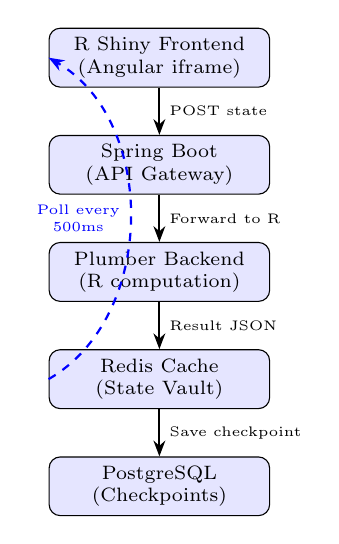
\begin{tikzpicture}[
    node distance=0.6cm,
    every node/.style={font=\scriptsize, align=center},
    box/.style={rectangle, draw, rounded corners, fill=blue!10, minimum width=2.8cm, minimum height=0.6cm},
    arrow/.style={-{Stealth[length=2mm]}, thick}
]
    \node[box] (shiny) {R Shiny Frontend\\(Angular iframe)};
    \node[box, below=of shiny] (spring) {Spring Boot\\(API Gateway)};
    \node[box, below=of spring] (plumber) {Plumber Backend\\(R computation)};
    \node[box, below=of plumber] (redis) {Redis Cache\\(State Vault)};
    \node[box, below=of redis] (pg) {PostgreSQL\\(Checkpoints)};
    
    \draw[arrow] (shiny) -- node[right, font=\tiny] {POST state} (spring);
    \draw[arrow] (spring) -- node[right, font=\tiny] {Forward to R} (plumber);
    \draw[arrow] (plumber) -- node[right, font=\tiny] {Result JSON} (redis);
    \draw[arrow] (redis) -- node[right, font=\tiny] {Save checkpoint} (pg);
    \draw[arrow, dashed, blue] (redis.west) to[bend right=60] node[left, font=\tiny, text=blue] {Poll every\\500ms} (shiny.west);
\end{tikzpicture}

\end{column}
\end{columns}

\end{frame}

% ============================================================
% SLIDE 7: RQ3 — ARCHITECTURE COMPARISON (DETAIL)
% ============================================================
\begin{frame}{RQ3: REST API vs.\ Event-Driven (Kafka) --- Trade-offs}

\begin{columns}[T]
\begin{column}{0.48\textwidth}

\textbf{REST API Architecture}
\begin{itemize}
    \item R backends run as \textbf{Plumber APIs} (HTTP endpoints)
    \item Spring Boot \textbf{routes requests} to correct Plumber service
    \item State stored in \textbf{Redis} (key-value cache)
    \item Frontends \textbf{poll} Redis via Spring Boot every 500ms
    \item Synchronous request--response model
\end{itemize}

\vspace{0.5em}
\textbf{Advantages:}
\begin{itemize}
    \item[\textcolor{green!60!black}{\faCheck}] Simpler infrastructure (no Kafka/Zookeeper)
    \item[\textcolor{green!60!black}{\faCheck}] Familiar HTTP semantics
    \item[\textcolor{green!60!black}{\faCheck}] Easier debugging (standard HTTP tools)
\end{itemize}

\textbf{Disadvantages:}
\begin{itemize}
    \item[\textcolor{red}{\faTimes}] Polling overhead (not true push)
    \item[\textcolor{red}{\faTimes}] Spring Boot is a bottleneck (single relay point)
\end{itemize}

\end{column}
\begin{column}{0.48\textwidth}

\textbf{Kafka Event-Driven Architecture}
\begin{itemize}
    \item R backends run as \textbf{standalone Kafka consumers}
    \item Direct \textbf{producer/consumer} communication via topics
    \item State flows through \textbf{input/output topics} (keyed by sessionId)
    \item Spring Boot only manages sessions, not data flow
    \item Asynchronous publish--subscribe model
\end{itemize}

\vspace{0.5em}
\textbf{Advantages:}
\begin{itemize}
    \item[\textcolor{green!60!black}{\faCheck}] Decoupled services (no central relay)
    \item[\textcolor{green!60!black}{\faCheck}] Natural event log (replayable)
    \item[\textcolor{green!60!black}{\faCheck}] Scales horizontally via partitions
\end{itemize}

\textbf{Disadvantages:}
\begin{itemize}
    \item[\textcolor{red}{\faTimes}] Heavier infrastructure (Kafka + Zookeeper)
    \item[\textcolor{red}{\faTimes}] R--Kafka integration is immature
\end{itemize}

\end{column}
\end{columns}

\end{frame}

% ============================================================
% SLIDE 8: RQ4 — BENCHMARKING METRICS (DETAIL)
% ============================================================
\begin{frame}{RQ4: How Will We Measure? --- Benchmarking Metrics}

\begin{columns}[T]
\begin{column}{0.55\textwidth}

\textbf{Three architectures under test:}
\begin{enumerate}
    \item \textbf{Monolithic Baseline} --- standard Shiny apps, no network, in-process computation
    \item \textbf{REST API} --- Plumber + Redis + Spring Boot relay
    \item \textbf{Kafka Event-Driven} --- Kafka topics + standalone R consumers
\end{enumerate}

\vspace{0.5em}
\textbf{Test Suite:} 8 R Shiny applications of varying complexity:
\begin{itemize}
    \item[\faCalculator] Calculator (minimal --- baseline latency)
    \item[\faChartBar] Visual Analytics (medium --- data filtering)
    \item[\faUpload] Data Exchange (I/O --- file upload + cleaning)
    \item[\faThermometerHalf] Climate Anomaly Detector (heavy --- 500K rows)
    \item[\faDice] Monte Carlo Simulator (CPU-bound)
    \item[\faMapMarkerAlt] Geospatial Editor (delta-based sync)
    \item[\faBrain] ML Trainer (long-running computation)
    \item[\faChartLine] Advanced Analytics (Plotly interactive)
\end{itemize}

\end{column}
\begin{column}{0.42\textwidth}

\begin{block}{\textbf{Metric 1: Latency}}
\small
End-to-end time from user input to UI update across all participants. Measured per-app, per-architecture.
\end{block}

\begin{block}{\textbf{Metric 2: Throughput / Speed}}
\small
Overall application performance, load times, and requests handled under concurrent users.
\end{block}

\begin{block}{\textbf{Metric 3: Data Loss}}
\small
Accuracy of state synchronisation. Do all participants receive every update? Are inputs/outputs consistent?
\end{block}

\begin{block}{\textbf{Metric 4: Cross-Contamination}}
\small
State leakage between parallel sessions. Does Session A's data ever appear in Session B?
\end{block}

\vspace{0.3em}
\small\textit{Automated via Playwright end-to-end tests.}

\end{column}
\end{columns}

\end{frame}

% ============================================================
% SLIDE 9: SUMMARY — RESEARCH QUESTIONS MAP
% ============================================================
\begin{frame}{Research Questions: How They Connect}

\begin{center}
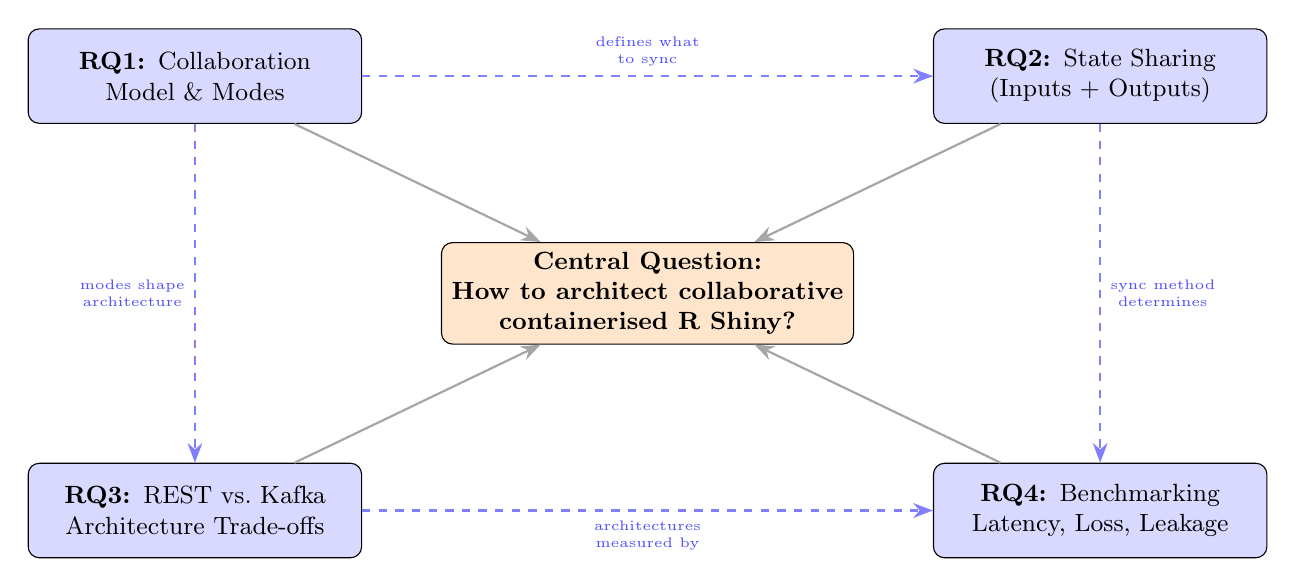
\begin{tikzpicture}[
    node distance=1.2cm and 2cm,
    every node/.style={font=\small, align=center},
    rq/.style={rectangle, draw, rounded corners=4pt, fill=blue!15, minimum width=4cm, minimum height=1.2cm, text width=4cm},
    central/.style={rectangle, draw, rounded corners=4pt, fill=orange!20, minimum width=5cm, minimum height=1.2cm, text width=5cm, font=\small\bfseries},
    arrow/.style={-{Stealth[length=2.5mm]}, thick, gray!70}
]
    % Central question
    \node[central] (cq) {Central Question:\\How to architect collaborative\\containerised R Shiny?};
    
    % RQs
    \node[rq, above left=1.5cm and 1cm of cq] (rq1) {\textbf{RQ1:} Collaboration\\Model \& Modes};
    \node[rq, above right=1.5cm and 1cm of cq] (rq2) {\textbf{RQ2:} State Sharing\\(Inputs + Outputs)};
    \node[rq, below left=1.5cm and 1cm of cq] (rq3) {\textbf{RQ3:} REST vs.\ Kafka\\Architecture Trade-offs};
    \node[rq, below right=1.5cm and 1cm of cq] (rq4) {\textbf{RQ4:} Benchmarking\\Latency, Loss, Leakage};
    
    % Arrows
    \draw[arrow] (rq1) -- (cq);
    \draw[arrow] (rq2) -- (cq);
    \draw[arrow] (rq3) -- (cq);
    \draw[arrow] (rq4) -- (cq);
    
    % Cross-links
    \draw[arrow, dashed, blue!50] (rq1) -- node[above, font=\tiny, text=blue!70] {defines what\\to sync} (rq2);
    \draw[arrow, dashed, blue!50] (rq2) -- node[right, font=\tiny, text=blue!70] {sync method\\determines} (rq4);
    \draw[arrow, dashed, blue!50] (rq3) -- node[below, font=\tiny, text=blue!70] {architectures\\measured by} (rq4);
    \draw[arrow, dashed, blue!50] (rq1) -- node[left, font=\tiny, text=blue!70] {modes shape\\architecture} (rq3);
    
\end{tikzpicture}
\end{center}

\vspace{0.5em}
\begin{center}
\small
RQ1 defines \textit{what} collaboration means $\rightarrow$ RQ2 defines \textit{what} to synchronise $\rightarrow$ RQ3 defines \textit{how} to synchronise $\rightarrow$ RQ4 measures \textit{how well} each approach works.
\end{center}

\end{frame}

\end{document}
